
We follow the discretisation presented in Section~\ref{ss:dgss1D} and use the 
successive substitution to arrive at the solution. 
Let us start by fixing ${\cal E}=4$ and ${\cal C}=0$ and setting the absolute convergence 
tolerance to $10^{-8}$.

\begin{center}
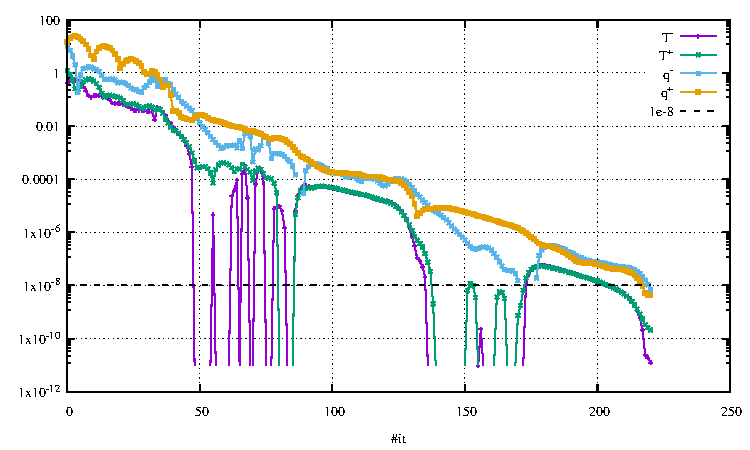
\includegraphics[width=8cm]{python_codes/fieldstone_57/results/E04_C000/convergence.pdf}
\end{center}

\begin{center}
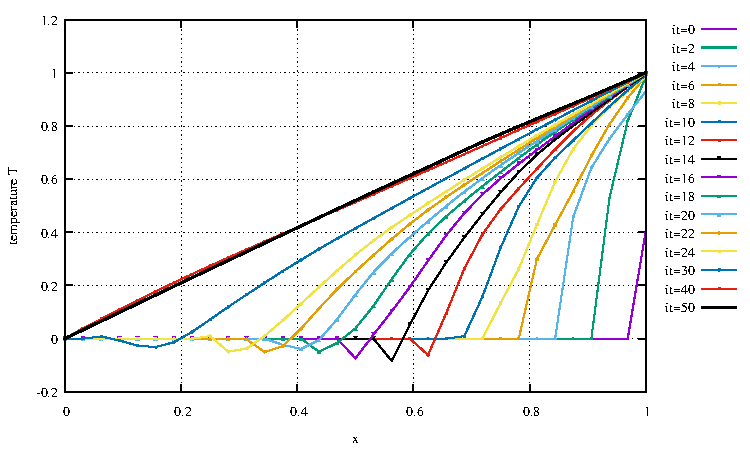
\includegraphics[width=7cm]{python_codes/fieldstone_57/results/E04_C000/T_minus_evol.pdf}
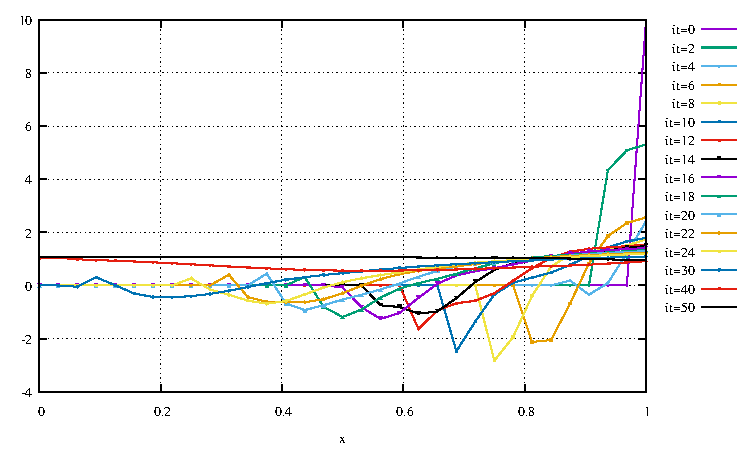
\includegraphics[width=7cm]{python_codes/fieldstone_57/results/E04_C000/q_minus_evol.pdf}
\end{center}

%...................................................
\paragraph{Effect of resolution} Keeping the same parameters we see that the 
number of required iterations to convergence increases linearly with the number of elements.

\begin{center}
\begin{tabular}{cc}
\hline
nelx & \# iterations \\
\hline
08 &60  \\
16 &116 \\
32 &220 \\
64 &436 \\
128 & 857 \\
\hline
\end{tabular}
\end{center}

%...................................................
\paragraph{Effect of ${\cal E}$ \& ${\cal C}$ values} 
We now keep nelx=32 and explore the effect of these parameters on the 
required number of iterations:

\begin{center}
\begin{tabular}{ccc}
\hline
${\cal E}$ & ${\cal C}$ & \# iterations \\
\hline
1& 0 & 772 \\
2& 0 & 414 \\
3& -0.5 & {\bf 104} \\
3& 0    & 284 \\
3& 0.5 & 129 \\
4&-1/2& 196 \\
4&0   & 220 \\
4&+1/2& 196 \\
5& -1/2 & 256 \\
5& 0 & 195 \\
5& +1/2 & 256 \\
6& 0 & 246 \\
10& 0 & 486 \\
\hline
\end{tabular}
\end{center}

\begin{center}
${\cal E}=4$ \& ${\cal C}=-1/2$  \hspace{2cm}
${\cal E}=4$ \& ${\cal C}=0$ \hspace{2cm}
${\cal E}=4$ \& ${\cal C}=+1/2$\\
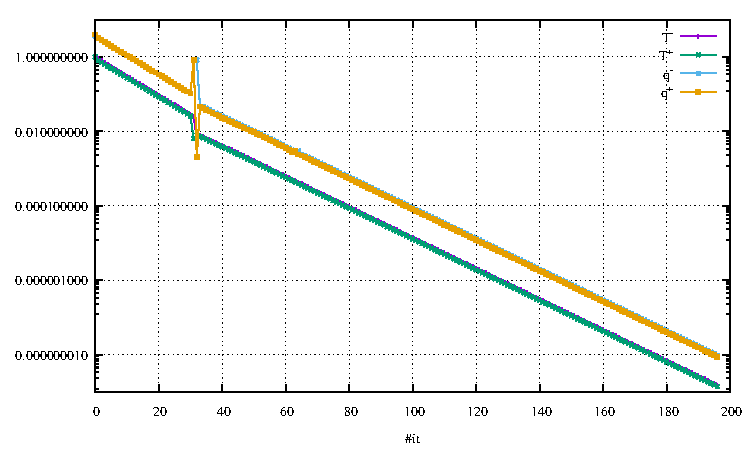
\includegraphics[width=5cm]{python_codes/fieldstone_57/results/E04_Cm0p5/convergence.pdf}
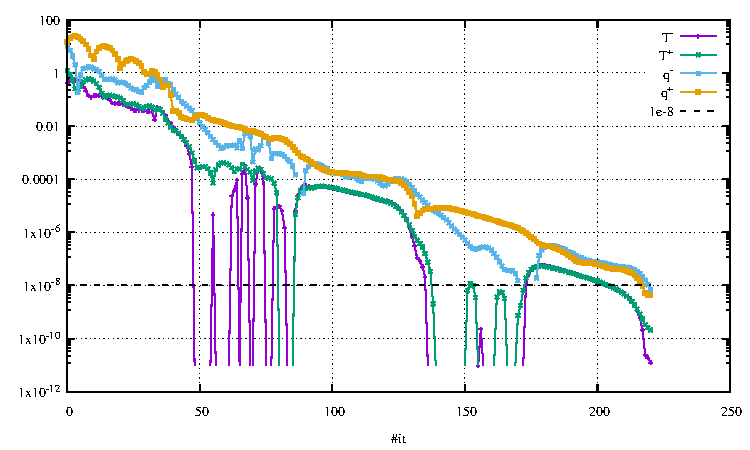
\includegraphics[width=5cm]{python_codes/fieldstone_57/results/E04_C000/convergence.pdf}
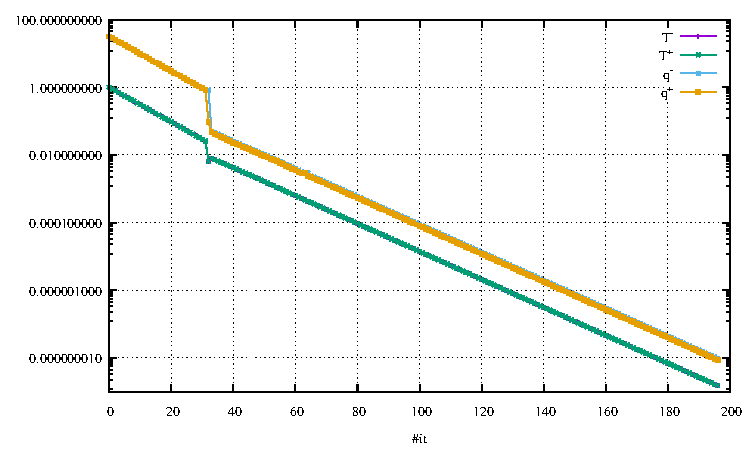
\includegraphics[width=5cm]{python_codes/fieldstone_57/results/E04_Cp0p5/convergence.pdf}\\
{\captionfont Using ${\cal C}\neq 0$ yields a very linear convergence.}
\end{center}


\begin{center}
${\cal E}=4$ \& ${\cal C}=-1/2$  \hspace{2cm}
${\cal E}=4$ \& ${\cal C}=0$ \hspace{2cm}
${\cal E}=4$ \& ${\cal C}=+1/2$\\
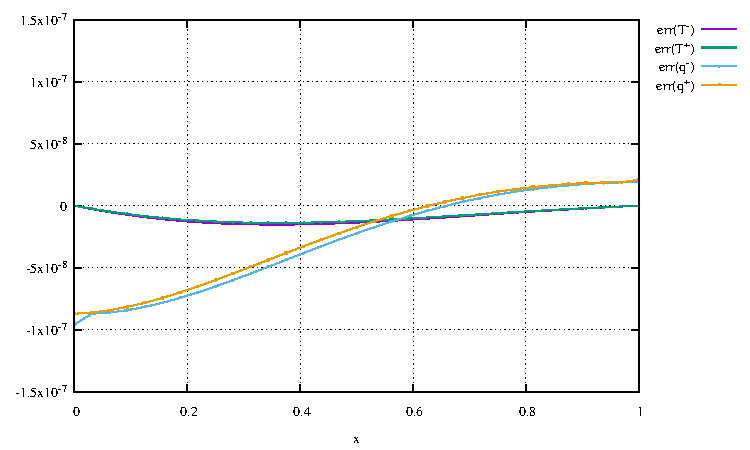
\includegraphics[width=5cm]{python_codes/fieldstone_57/results/E04_Cm0p5/error.pdf}
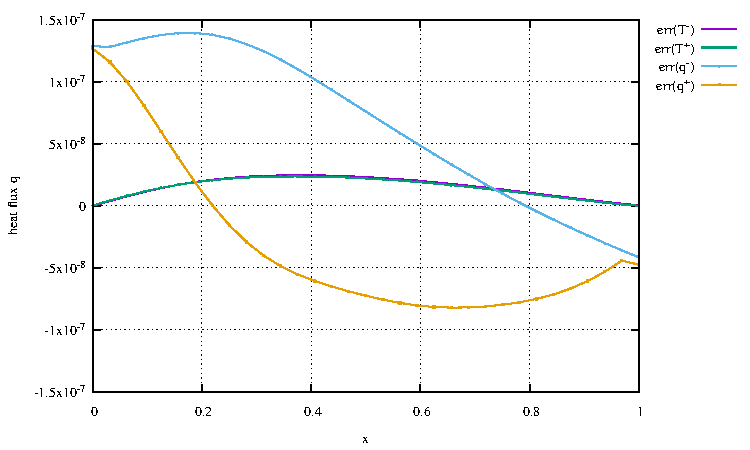
\includegraphics[width=5cm]{python_codes/fieldstone_57/results/E04_C000/error.pdf}
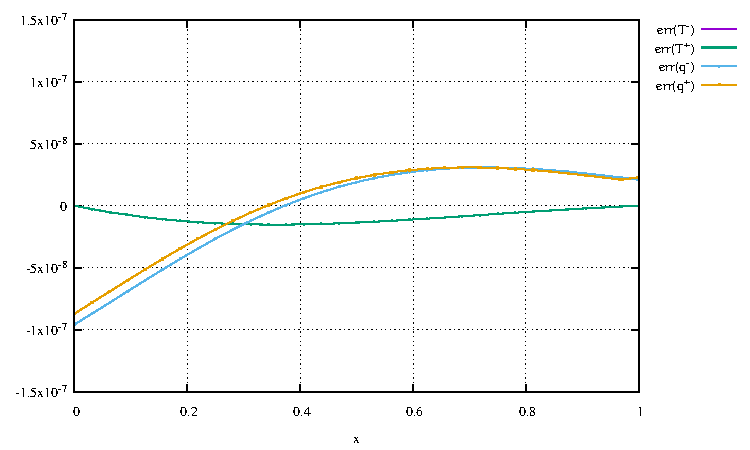
\includegraphics[width=5cm]{python_codes/fieldstone_57/results/E04_Cp0p5/error.pdf}\\
{\captionfont Error between computed and analytical solution as a function of $x$} 
\end{center}


\begin{center}
${\cal E}=4$ \& ${\cal C}=-1/2$  \hspace{2cm}
${\cal E}=4$ \& ${\cal C}=0$ \hspace{2cm}
${\cal E}=4$ \& ${\cal C}=+1/2$\\
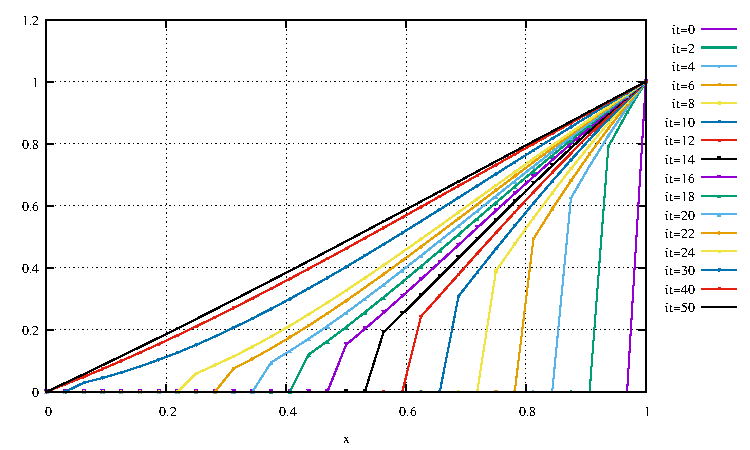
\includegraphics[width=5cm]{python_codes/fieldstone_57/results/E04_Cm0p5/T_minus_evol}
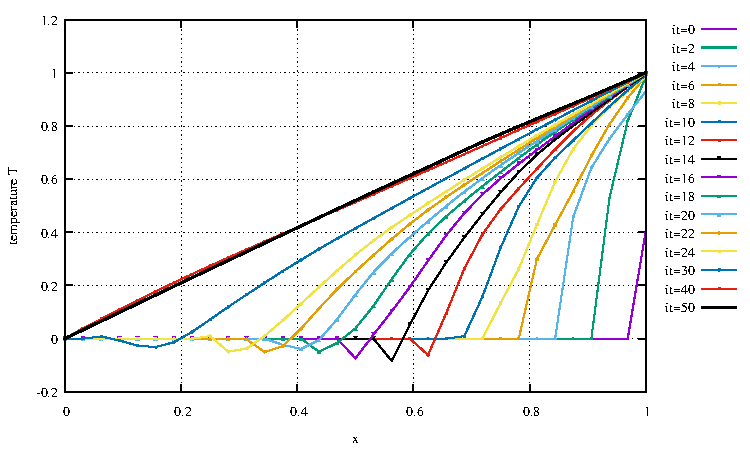
\includegraphics[width=5cm]{python_codes/fieldstone_57/results/E04_C000/T_minus_evol}
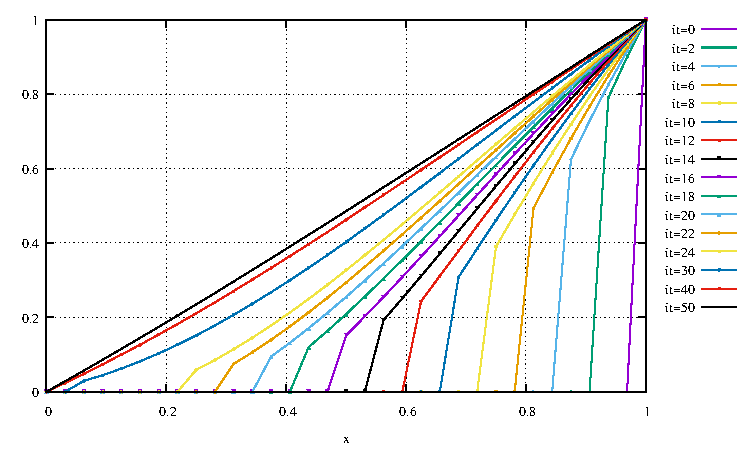
\includegraphics[width=5cm]{python_codes/fieldstone_57/results/E04_Cp0p5/T_minus_evol}\\
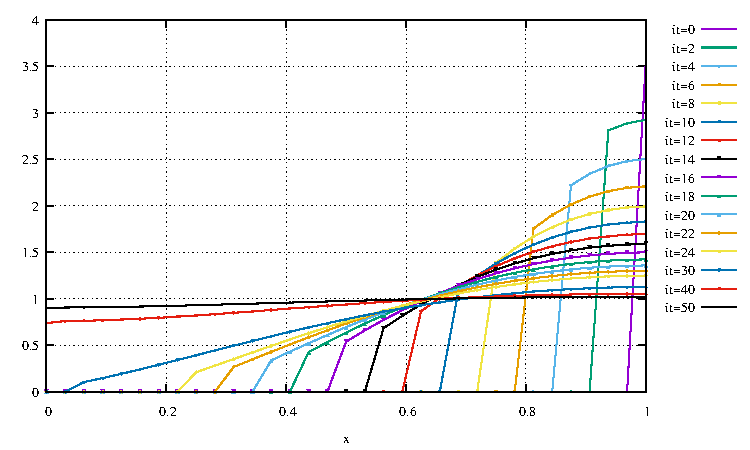
\includegraphics[width=5cm]{python_codes/fieldstone_57/results/E04_Cm0p5/q_minus_evol}
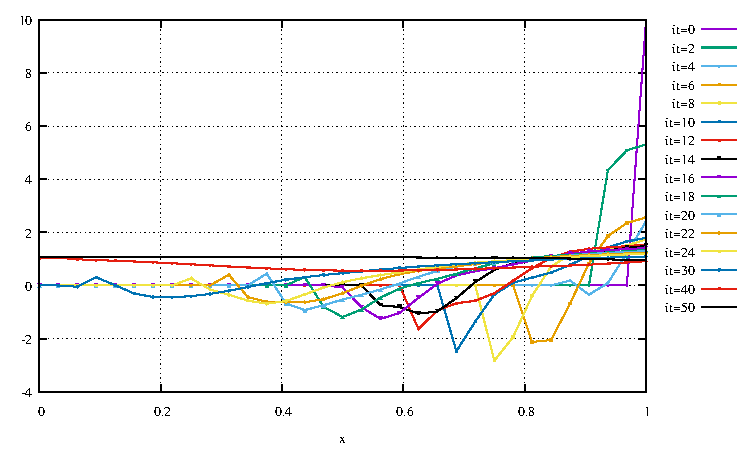
\includegraphics[width=5cm]{python_codes/fieldstone_57/results/E04_C000/q_minus_evol}
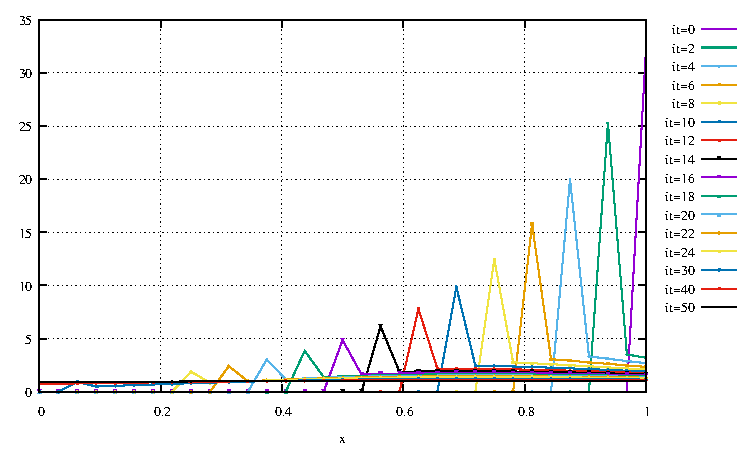
\includegraphics[width=5cm]{python_codes/fieldstone_57/results/E04_Cp0p5/q_minus_evol}\\
{\captionfont The path to a converged solution is quite different for the three values 
of ${\cal C}$ tested.} 
\end{center}




